\documentclass[11pt]{scrartcl}
\usepackage[utf8]{inputenc}
\usepackage{enumitem}
\usepackage{amsfonts}
\usepackage{bbm}
\usepackage{newtxmath}
%\usepackage[square]{natbib}
\usepackage{amsmath}
\usepackage{mathrsfs,bm}
\usepackage{graphicx,epstopdf,caption}
\usepackage{float,subcaption,setspace,booktabs,multirow,supertabular,lscape,threeparttable}
\usepackage{float,colortbl}
\usepackage{placeins}
\usepackage{indentfirst}
\usepackage{enumitem}
\setlength{\parindent}{0pt} %% noindent for the entire file % or add indent {2em}
\usepackage{geometry}
\geometry{left=0.8in,right=0.8in,top=1in,bottom=0.5in}
\usepackage[noblocks]{authblk}
\usepackage{lipsum}%% a garbage package you don't need except to create examples.
\usepackage{fancyhdr}
\usepackage[svgnames]{xcolor}
\usepackage{listings}
\usepackage{verbatim}
\usepackage[round, semicolon, sort]{natbib}
\setlength{\parindent}{2em}
\usepackage[font={footnotesize, it}]{caption}

\pagestyle{fancy}
\lhead{CSCI 5561}  % set your name here
\chead{\large\textbf{Homework 4 - CNN}}
\rhead{He Zhou (zhou1354@umn.edu)}
\renewcommand{\headrulewidth}{0.4pt}

\lstset{language=R,
	basicstyle=\small\ttfamily,
	stringstyle=\color{DarkGreen},
	otherkeywords={0,1,2,3,4,5,6,7,8,9},
	morekeywords={TRUE,FALSE},
	deletekeywords={data,frame,length,as,character},
	keywordstyle=\color{blue},
	commentstyle=\color{DarkGreen},
}
\usepackage{Sweave}
\graphicspath{{Figures/}}  % set the path of figures
\usepackage{blindtext}
\usepackage{scrextend}
\addtokomafont{labelinglabel}{\bfseries}
\usepackage{appendix}
\usepackage[linesnumbered,ruled,vlined]{algorithm2e}

\usepackage{algpseudocode}  
\usepackage{hyperref}
\hypersetup{
    colorlinks=true,
    linkcolor=blue,
    filecolor=blue,      
    urlcolor=blue,
    citecolor=cyan,
}

\newcommand{\cX}{\mathcal{X}}
\newcommand{\cR}{\mathcal{R}}
\newcommand{\cV}{\mathcal{V}}
\newcommand{\bw}{\mathbf{w}}

	

\begin{document}

\title{CSCI 5561}
\author{\Large Homework 4 -- Convolutional Neural Network\\
	He Zhou}  %% set your name on the main page
%\date{\vspace{-5ex}}  % suppress the output of date
\maketitle
\newpage
\paragraph{\textbf{MNIST Data: }}
The goal of this assignment is to implement a single-layer linear perceptron, a single-layer perceptron, a multi-layer perceptron and a convolutional neural network to recognize hand-written digits in the MNIST dataset. The size of each image is $196=14\times 14$ with a label in $\{0,1,2,\cdots, 9\}$. For each neural network, the stochastic gradient descent method will be implemented to optimize the objective function $\sum_{i=1}^{n}\ell(y_i,f(x_i;\bm{\theta}))$, 
where $\ell()$ is the loss function and $\{f(\cdot;\bm{\theta})\}$ is the family of function with coefficient $\bm{\theta}$.

\paragraph{\textbf{List of Functions: }}
\texttt{get\_mini\_batch()}: randomly permutes the order of images to build the mini-batch of size $\texttt{batch\_size}=32$ for stochastic gradient descent. Each batch of images is a matrix with size $196\times\texttt{batch\_size}$, and each batch of labels is a matrix with size $10\times\texttt{batch\_size}$, where the labels are converted to $\{0,1\}^{10}$ using one-hot encoding.
\\
\indent\texttt{fc()} and \texttt{fc\_backward()}: \texttt{fc} is the fully connected layer, i.e., a linear transform of $\mathbf{x}\in\mathbb{R}^{n\times1}$: $\mathbf{y}=\mathbf{w}\mathbf{x}+\mathbf{b}$, where $\mathbf{w}\in\mathbb{R}^{m\times n}$ and $\mathbf{b}\in\mathbb{R}^{m\times 1}$. \texttt{fc\_backward} computes the partial derivative w.r.t. input $\mathbf{x}$, weights $\mathbf{w}$, and bias $\mathbf{b}$ using the loss derivative w.r.t. the output $\mathbf{y}$. 
	\\
\indent\texttt{loss\_euclidean()}: Compute the Euclidean distance $L=\Vert\mathbf{y}-\tilde{\mathbf{y}}\Vert^2$  and the loss derivative w.r.t. the prediction $\texttt{y\_tilde}$, i.e., $2(\tilde{\mathbf{y}}-\mathbf{y})$.
\\
\indent\texttt{loss\_cross\_entropy\_softmax()}: Add a soft-max layer to input $\mathbf{x}$, i.e., $\tilde{y}_j={e^{x_j}}/{(\sum_{j}e^{x_j})}$ and compute the cross-entropy between the two distributions $L=-\sum_{j=1}^{m}y_j\log\left(\tilde{y}_j\right)$. The loss derivative w.r.t. the input $\mathbf{x}$ is $\tilde{\mathbf{y}}-\mathbf{y}$.
\\
\indent \texttt{relu()} and \texttt{relu\_backward()}: \texttt{relu} is an activation unit, $\max(\cdot,0)$. \texttt{relu\_backward} computes the loss derivative w.r.t. the relu input $\mathbf{x}$: $\frac{\partial L}{\partial\mathbf{x}}=\frac{\partial L}{\partial\mathbf{y}}\cdot I\{\mathbf{x}>0\}$.
\\
\indent\texttt{conv()} and \texttt{conv\_backward()}: \texttt{conv} is a convolutional operation with weights $\texttt{w\_conv}\in\mathbb{R}^{h\times w\times C_1\times C_2}$ and bias $\texttt{b\_conv}\in\mathbb{R}^{C_2\times 1}$. Zeros are padded at the boundary of the input image. \texttt{conv\_backward} computes the loss derivatives w.r.t. the weights and bias. We employ the \texttt{im2col} and \texttt{col2im}\footnote{\url{https://leonardoaraujosantos.gitbook.io/artificial-inteligence/machine_learning/deep_learning/convolution_layer/making_faster}}  operations that convert the convolution operation into a matrix multiplication to simplify the computation.
\\
\indent\texttt{pool2x2()} and \texttt{pool2x2\_backward()}: $2\times 2$ max-pooling operation and its loss derivative w.r.t. the input.
\\
\indent\texttt{flattening()} and \texttt{flattening\_backward()}: Flattening operation and its loss derivative w.r.t. the input.


\paragraph{\textbf{Single-layer Linear Perceptron:}}
Function \texttt{train\_slp\_linear} with functions  \texttt{fc}, \texttt{fc\_backward} and \texttt{loss\_euclidean} implements a single layer linear perceptron with stochastic gradient descent method. The function $f()$ for this single-layer linear perceptron is a fully connected layer: $\sigma_{\text{fc}}(\mathbf{x};\mathbf{w},\mathbf{b})=\mathbf{wx}+\mathbf{b}$. The loss function is the Euclidean loss: $\ell(\mathbf{y},\tilde{\mathbf{y}})=\Vert\mathbf{y}-\tilde{\mathbf{y}}\Vert^2$. When implementing the stochastic gradient descent method, the learning rate and the decaying rate are tuned as $\gamma=0.01$, $\lambda=0.1$, and the maximum number of iterations is $\textit{nIters}=2000$.  The visualization of confusion matrix is given in Figure (1a) and the accuracy of the prediction is  $0.296$. We can see that the single-layer linear perceptron does not perform well.


\begin{figure}[H]
	\captionsetup[subfigure]{labelformat=empty}
	\centering
	\subcaptionbox{(1a) Single-layer linear perceptron}{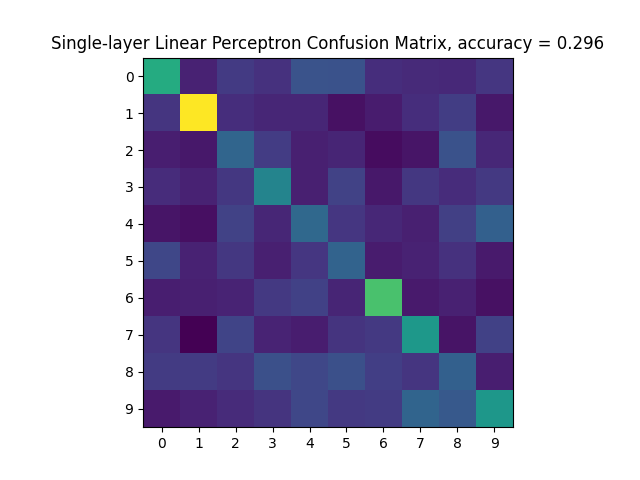
\includegraphics[height=4.5cm,keepaspectratio]{slp_linear_confusion.jpg}}
	\subcaptionbox{(1b) Single-layer perceptron}{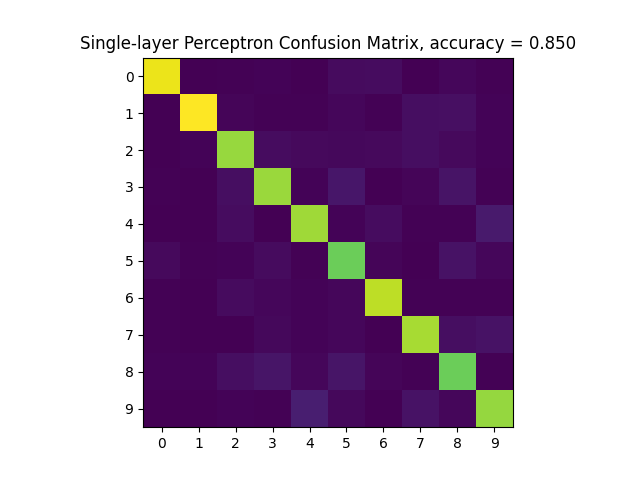
\includegraphics[height=4.5cm,keepaspectratio]{slp_confusion.jpg}}
	\label{fig:slp_linear}
\end{figure}

\paragraph{\textbf{Single-layer Perceptron:}} 
The single-layer perceptron (\texttt{train\_slp}) adds a soft-max layer to the previous single-layer perceptron and uses the cross-entropy as the loss function: $f(\mathbf{x};\mathbf{w},\mathbf{b})=\sigma_{\text{soft\_max}}(\sigma_{\text{fc}}(\mathbf{x};\mathbf{w},\mathbf{b}))$, $\ell(\mathbf{y},\tilde{\mathbf{y}})=-\sum_{j=1}^{m}y_j\log\left(\tilde{y}_j\right)$. When implementing the stochastic gradient descent method, the learning rate and the decaying rate are tuned as $\gamma=0.135$, $\lambda=0.895$, and the maximum number of iterations is $\textit{nIters}=2500$. The visualization of confusion matrix is given in Figure (1b) and the accuracy of the prediction is  $0.850$. We can see that the single-layer perceptron performs much better than the single-layer linear perceptron.



\paragraph{\textbf{Multi-layer Perceptron:}}
The multi-layer perceptron (\texttt{train\_mlp}) implements a fully-connected layer, a relu layer, another fully-connected layer, and a soft-max layer sequentially with the cross-entropy loss, shown in Figure (2a). $$f(\mathbf{x};\mathbf{w}_1,\mathbf{b}_1,\mathbf{w}_2,\mathbf{b}_2)=\sigma_{\text{soft\_max}}(\sigma_{\text{fc}}(\sigma_{\text{relu}}(\sigma_{\texttt{fc}}(\mathbf{x};\mathbf{w}_1,\mathbf{b}_1));\mathbf{w}_2,\mathbf{b}_2)).
$$
The back-propergation algorithm is implemented to calculate the partial derivatives w.r.t. the coefficients. When implementing the stochastic gradient descent method, the learning rate and the decaying rate are tuned as $\gamma=0.49$, $\lambda=0.905$, and the maximum number of iterations is $\textit{nIters}=5000$. The visualization of confusion matrix is given in Figure (2b) and the accuracy of the prediction is $0.904$. We can see that adding a relu layer and a second fully-connected layer improves the prediction accuracy. 



\begin{figure}[H]
	\captionsetup[subfigure]{labelformat=empty}
	\centering
	\subcaptionbox{(2a) Multiple-layer perceptron}{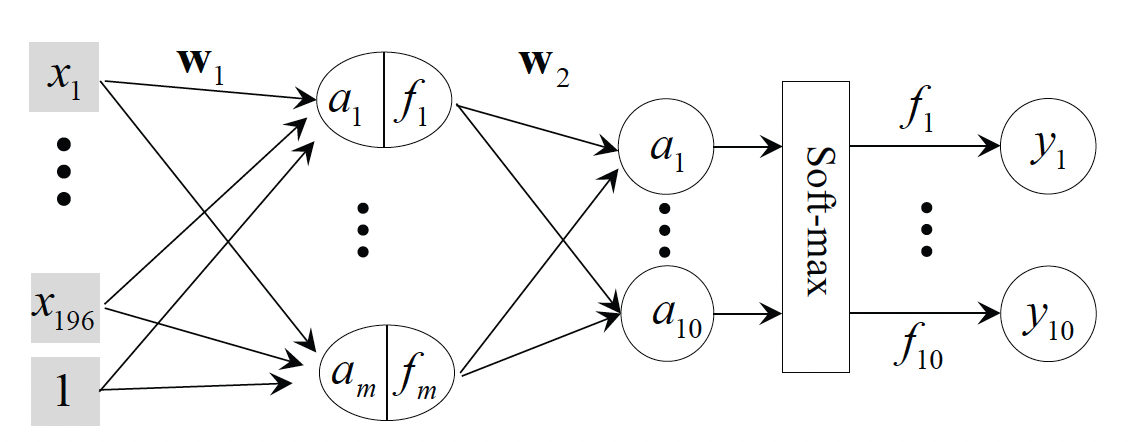
\includegraphics[height=3.5cm,keepaspectratio]{mlp.png}}
	\subcaptionbox{(2b) Confusion matrix with accuracy $0.904$}{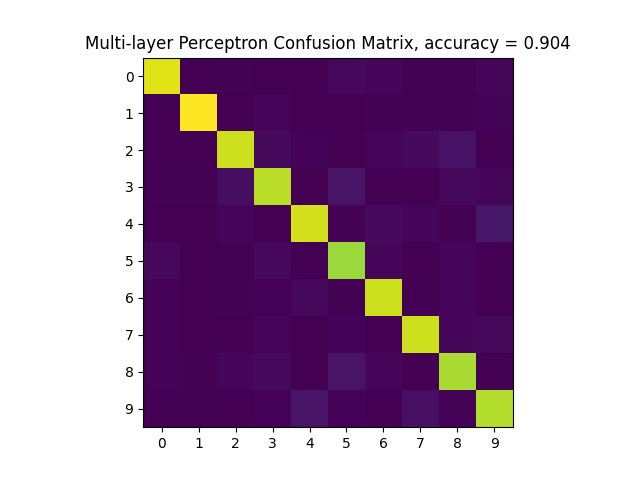
\includegraphics[height=4.5cm,keepaspectratio]{mlp_confusion.jpg}}
	\label{fig:mlp}
\end{figure}


\paragraph{\textbf{Convolutional Neural Network:}}
The CNN (\texttt{train\_cnn}) is composed of a single channel input ($14\times 14\times1$) $\rightarrow$ the convolutional layer ($3\time3$ convolution with $3$ channels and stride $1$) $\rightarrow$ ReLu layer $\rightarrow$ Max-pooling layer ($2\times2$ with stride $2$) $\rightarrow$ Flattening layer $\rightarrow$ Fully-connected layer $\rightarrow$ Soft-max layer, shown in Figure (3a). 
$$
f(\mathbf{x};\texttt{w\_conv},\texttt{b\_conv},\texttt{w\_fc},\texttt{b\_fc})=\sigma_{\text{soft\_max}}(\sigma_{\text{fc}}(\sigma_{\text{flat}}\circ\sigma_{\text{pool}}\circ\sigma_{\text{relu}}\circ\sigma_{\text{conv}}(\mathbf{x};\texttt{w\_conv},\texttt{b\_conv});\texttt{w\_fc},\texttt{b\_fc}))
$$
The back-propergation algorithm is implemented to calculate the partial derivatives w.r.t. the coefficients. When implementing the stochastic gradient descent method, the learning rate and the decaying rate are tuned as $\gamma=0.5$, $\lambda=0.89$, and the maximum number of iterations is $\textit{nIters}=1000$. The visualization of confusion matrix is given in Figure (3b) and the accuracy of the prediction is $0.924$. We can see that implementing a CNN could further improve the prediction accuracy. 




\begin{figure}[H]
	\captionsetup[subfigure]{labelformat=empty}
	\centering
	\subcaptionbox{(3a) Convolutional neural network perceptron}{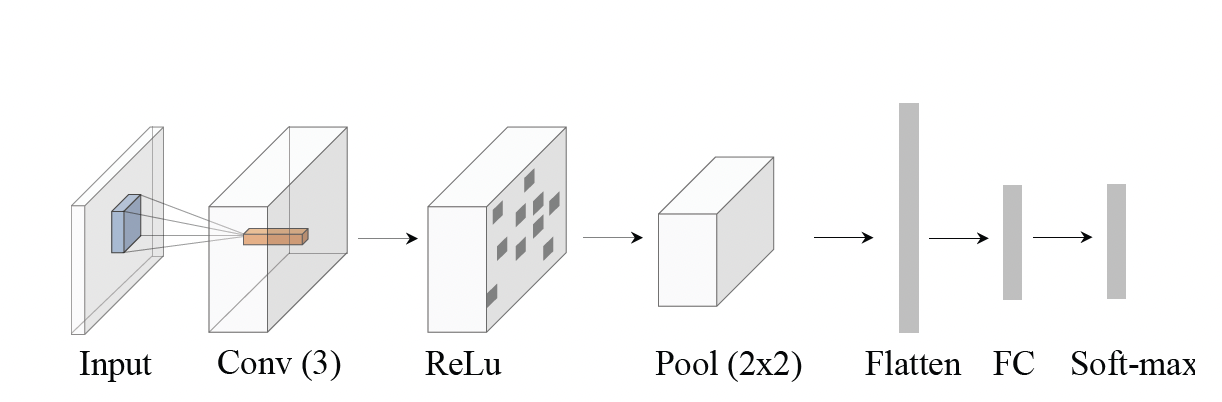
\includegraphics[height=3.4cm,keepaspectratio]{cnn.png}}
	\subcaptionbox{(3b) Confusion matrix with accuracy $0.924$}{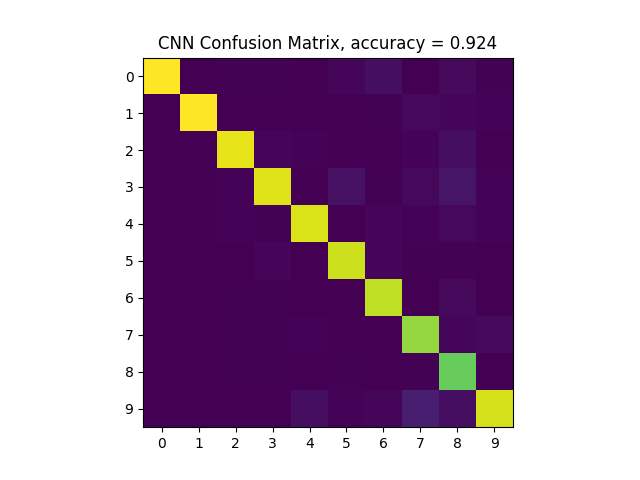
\includegraphics[height=4.4cm,keepaspectratio]{cnn_confusion.jpg}}
	\label{fig:cnn}
\end{figure}














\nocite*{}  
%\bibliographystyle{apalike}  %disordered
%\bibliographystyle{plain}  %ordered by auther
%\bibliographystyle{unsrt}  %ordered as referenced
\bibliographystyle{IEEEtranN}
\bibliography{bibfile}






\end{document}